\subsection{Objeto}

Um objeto é uma estrutura dinâmica construída com base em uma classe. Sendo que,
com base em uma classe é possível criar vários objetos, cada qual com suas
propriedades \cite{phpProgramandoComOrientacaoAObjetos}.

De forma breve, os objetos são as instâncias de uma classe. Sendo que, as
classes existem somente no código fonte de uma aplicação, enquanto que, as
instâncias de uma classe existem durante a execução de um programa. Portanto,
o software poderá criar vários objetos sob demanda tendo como base um mesmo
modelo \cite{ios7ProgrammingFundamentalsObjectiveCXcodeAndCocoaBasics}. Deste
modo, esses objetos são criados (instanciados) através de métodos construtores
e destruídos (eliminados) através de métodos destrutores em tempo de execução
\cite{umlEC++GuiaPraticoDeDesenvolvimentoOrientadoAObjeto}. Será apresentado no
decorrer deste capítulo como funcionam os métodos construtores e destrutores.

\begin{figure}[h!tb]
	\caption{Criação de um objeto na linguagem PHP}
	\label{fig:objeto}

	\centering
	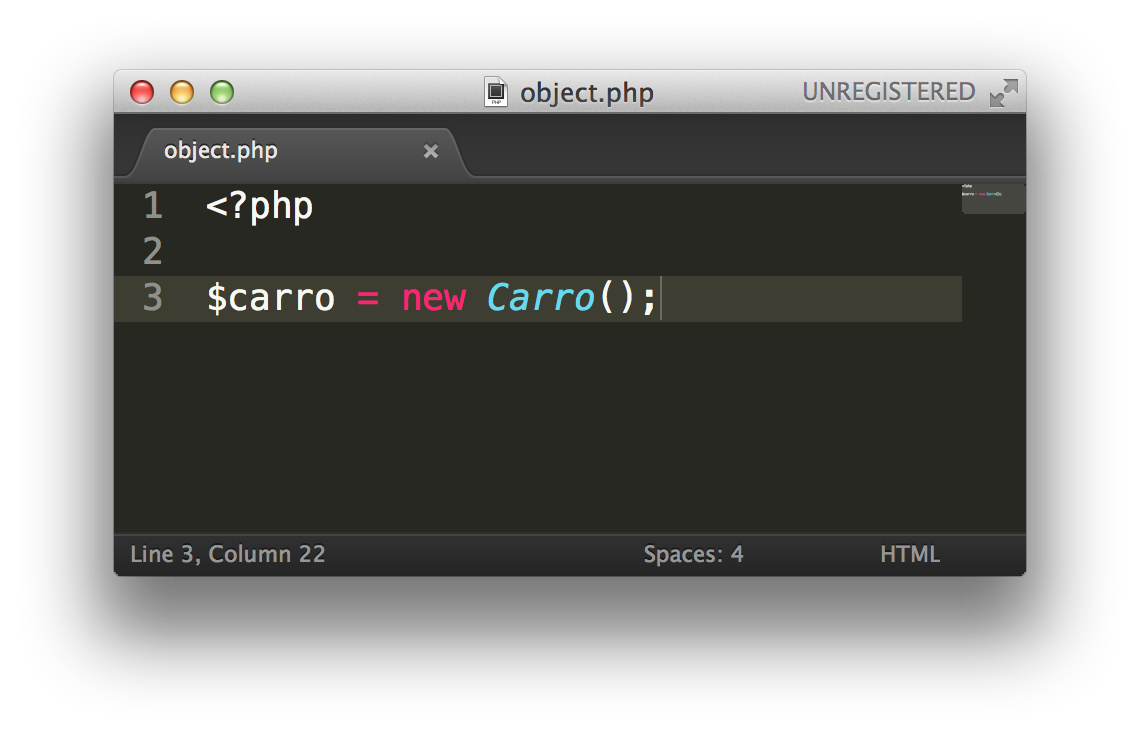
\includegraphics[width=0.65\textwidth]{images/object.png}

	\centering
	\footnotesize Fonte: \fonteOAutor
\end{figure}

\FloatBarrier 	% Este comando impede que as imagens
				% flutuem a partir deste ponto no seu documento

A seguir, será apresentada a análise do código exibido na
Figura \ref{fig:objeto}:

\begin{alineas}
    \item linha 1: tem-se o início da execução de um bloco de código PHP;
    \item linha 3: é definida uma variável chamada \textbf{\$carro};
    chama-se um operador de atribuição da linguagem (representado pelo símbolo
    \textbf{=}) que irá atribuir o valor que está à direita do operador na
    variável que está à esquerda; em seguida é informado um outro operador da
    linguagem (representado pelo símbolo \textbf{new}) que é responsável por
    criar uma referência em memória para o tipo de dados que está sendo
    criado e, por fim, define-se a classe que deverá ser instanciada, que neste
    caso, chama-se Carro. Logo após, o símbolo \textbf{()} representa um método
    construtor (conceito que será apresentado ainda neste capítulo de Orientação
    a Objetos).
    Uma informação importante é que toda instrução da linguagem \acs{PHP} termina
    com o símbolo de ponto-e-vírgula.
\end{alineas}